\documentclass{article}

\usepackage{amsmath}
\usepackage{amssymb}
\usepackage{parskip}
\usepackage{fullpage}
\usepackage{graphicx}
\usepackage{hyperref}
\usepackage{listings}
\usepackage{xcolor}
\usepackage{listings-rust}

\hypersetup{
    colorlinks=true,
    linkcolor=black,
    urlcolor=blue,
    pdftitle={Paolo Bettelini - Diaries},
    pdfpagemode=FullScreen,
}

\definecolor{background}{HTML}{EEEEEE}

\lstdefinestyle{generic} {
    backgroundcolor=\color{background},
    numbers=none,
    basicstyle=\ttfamily\color{black},
    breaklines=true,
    frame=lines
}

\title{Diaries}
\author{Paolo Bettelini}
\date{}

\begin{document}

\maketitle
\tableofcontents
\pagebreak

\section{Diaries}

\subsection{2022-12-13}

Work hours:\\
\textbf{08:20 - 11:15}: Setup and research

Today I setup the git repository with the initial files
(CLI tool, documentation, etc.).
I then spent the rest of the working
session researching the topic of the project.

The planning has yet to be done.
The goal for the next working session is to make the Gantt chart.

\subsection{2022-12-14}

Work hours:\\
\textbf{15:10 - 16:20}: Alpha matting test \\
\textbf{16:00 - 16:20}: Gantt chart

Today I started using the \texttt{opencv} library (The Rust wrapper).
I used the sample images (target and trimap) from \href{https://docs.opencv.org/4.x/dd/d0e/tutorial\_alphamat.html}{https://docs.opencv.org/4.x/dd/d0e/tutorial\_alphamat.html}.
The output is not correct, but it shows some matting to be applied.
\begin{figure}[h]
    \centering
    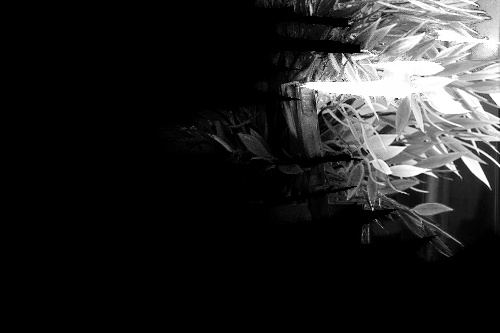
\includegraphics[width=0.75\textwidth]{res1}
\end{figure}

However, I noticed a small problem: when the input images are
wrong, instead of returning \texttt{Result(Err)} (as per Rust-philosophy),
it dumps the core.

I also started making the Gantt chart.

\pagebreak

\subsection{2022-12-15}

Work hours:\\
\textbf{08:20 - 09:50}: CLI executable \\
\textbf{10:20 - 11:20}: Gantt chart

Today I fixed the trimap matting. The trimap was being read using
\texttt{IMREAD\_COLOR} rather than \texttt{IMREAD\_GRAYSCALE}.
I then added the first CLI arguments to the executabl (target image,
trimap image, output image).
I need to find a solution to avoid the core dumps from \texttt{opencv}.

\begin{figure}[h]
    \centering
    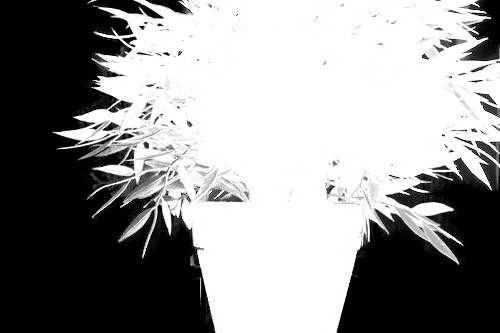
\includegraphics[width=0.75\textwidth]{res2}
\end{figure}

In the second half of the working session I completed the gantt chart

\subsection{2022-12-20}

Work hours:\\
\textbf{08:20 - 09:50}: OpenCV documentation \\
\textbf{10:20 - 11:20}: Documentation and requirements

In the first half of the working session I read
some documentation about OpenCV.
The goal is to be able to remove the background of an image
given its trimap.
In the second half I continued setting up the documentation
(requirements and layout).

\subsection{2022-12-21}

Work hours:\\
\textbf{15:05 - 15:30}: Documentation \\

Today I continued the analysis section.

\subsection{2022-12-22}

Work hours:\\
\textbf{08:20 - 09:50}: Background removal research \\
\textbf{10:05 - 10:30}: Read the review of my previous project documentation \\
\textbf{10:30 - 11:20}: GUI Research

Today I did not write any actual code, however, I did some research on which
technologies I will need to use. I realized that the background removal
cannot be done using \texttt{opencv}, but rather with another library.
Not much effort is necessary in order to finish the CLI tool, so I started
looking into the Rust GUI libraries. I also conitnued writing the requirements
in the analysis section.

The plan for the next working session is to finish the CLI tool.

\subsection{2023-01-09}

Work hours:\\
\textbf{13:15 - 16:30}: CLI

Within the last week I completed the CLI tool.
The CLI tool is capable of genering soft masks given trimaps.
It can also apply operations to images such as: making the background transparent,
filling the background with a color or replacing the background with another image.

\begin{lstlisting}[style=generic]
    Matting CLI
    
    Usage: matting-cli [OPTIONS] --target <TARGET> <--mask <MASK>|--trimap <TRIMAP>>
    
    Options:
      -i, --target <TARGET>        Target image
          --mask <MASK>            Background mask image
          --trimap <TRIMAP>        Trimap image
          --save-mask <SAVE_MASK>  Save mask path
      -o, --output <OUTPUT>        Output image
      -f, --fill <FILL>            Fill background action
      -t, --transparent            Transparent background action
      -r, --replace <REPLACE>      Replace background action
      -h, --help                   Print help information
      -V, --version                Print version information
\end{lstlisting}

The CLI tool still lacks error handling. \\
Another feature to add is the \texttt{--verbose} flag,
which prints what the program is doing along with timestamps.

\subsection{2023-01-10}

Work hours:\\
\textbf{08:20 - 9:50}: Error handling \\
\textbf{10:05 - 11:00}: Verbose flag

Today I handled every possible crash in the CLI tool.
Whenever an errors occurs it prints the according message.
I also started implemented the \texttt{--verbose} flag,
which prints program statuses and timestamps.

The plan for the next working session is to finish implementing the verbose flag.
Next, the server application can be developed.

\subsection{2023-01-11}

Work hours:\\
\textbf{15:00 - 16:20}: Verbose flag and refactor

Today I continued implementing the \texttt{--verbose} flag.
The CLI tool now prints what it is doing, but I haven't implemented the timestampts yet.
I also did some refactoring of the code and cleanup.

\subsection{2023-01-12}

Work hours:\\
\textbf{08:30 - 09:50}: CLI timestamps \\
\textbf{10:05 - 11:20}: Documentation

The CLI now fully supports the \texttt{--verbose} flag
and prints the elapsed time for each operation.

\begin{lstlisting}[style=boxed]
> matting-cli -i target.jpg --trimap trimap.png --save-mask mask.png
    --verbose -o out.png --fill red

Reading target image... Done! [4.021485ms]
Reading trimap image... Done! [1.976477ms]
Generating soft mask... Done! [7.104532642s]
Reading target image... Done! [178.884124ms]
Saving soft mask... Done! [509.050896ms]
Filling background with color... Done! [117.90393ms]
Saving output... Done! [954.085622ms]
\end{lstlisting}

I created the \lstinline[style=Rust]{log!()} macro which executes
an expression and logs a message and the elapsed time if a given flag is true.

\begin{lstlisting}[style=Rust, style=boxed]
    let mask = log!(
        "Generating soft mask",
        args.verbose,
        matting::generate_mask(&target, &trimap)? // heavy lifting
    );
\end{lstlisting}

In the second half of the working session I continued the documentation.
I did not write any actual documentation, just boilerplate and useful stuff that I'll be using.

The plan for the next working session is to crate the server worker.

\subsection{2023-01-17}

Work hours:\\
\textbf{08:30 - 11:20}: Server and API

Today I starting implementing the backend worker to process
the images. The route still does not work, althought the development
of the webserver should go smoothly after this issue.

The plan for the next working session is to continue the documentation.

\subsection{2023-01-18}

Work hours:\\
\textbf{15:00 - 16:20}: Documentation

Today I continued the documentation. I wrote the
following sections:
\begin{enumerate}
    \item \texttt{Introduction/Information}
    \item \texttt{Trimap Matting}
\end{enumerate}

\subsection{2023-01-19}

Work hours:\\
\textbf{08:30 - 10:40}: Webserver \\
\textbf{10:40 - 11:00}: Helped a classmate \\
\textbf{11:00 - 11:20}: Documentation

Today I continued working on the backend. The webserver
now serves the static webistes files. The upload root
can read the image data.

I also continued the documentation and wrote a small section
about OpenCV (\texttt{OpenCV}).

\subsection{2023-01-23}

Work hours:\\
\textbf{13:20 - 16:20}: Webserver and frontend

Today I continued working on the backend and the frontend.
The backend successfully receives POST requests containing an image
and can read its data. The frontend can load images onto the canvas
and send the canvas contents to the server. I also started
implementing the brush feature. The canvas is already capable
of simple painting features.

\subsection{2023-01-24}

Work hours:\\
\textbf{08:30 - 11:20}: Frontend Trimap Painting

Today I focused on implementing the painting feature on the frontend. \\
When an image is uploaded, I can start painting over it. There are a few settings and features such as:
\begin{itemize}
    \item Brush size slider
    \item Background / Forground selection
    \item Opacity slider
    \item Undo action
    \item Clear canvas action
\end{itemize}

I still need to implement the redo feature, and the undo features does not work if the clear feature has been
used previously. The plan for the next working session is to solely continue the documentation.

\begin{figure}[h]
    \begin{minipage}{0.5\textwidth}
        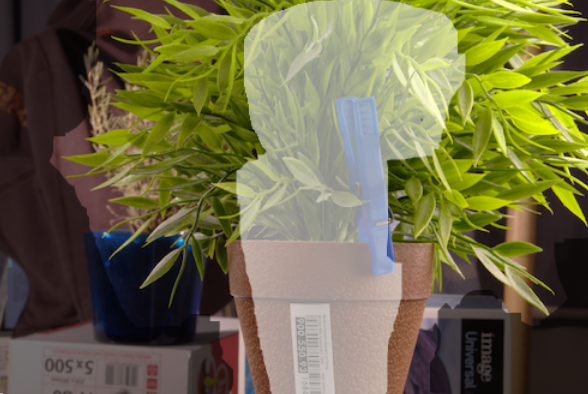
\includegraphics[width=\textwidth]{painting1.png}
    \end{minipage}
    \begin{minipage}{0.5\textwidth}
        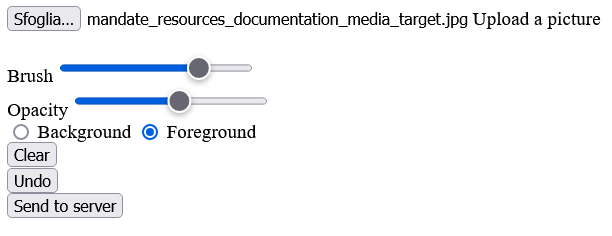
\includegraphics[width=\textwidth]{painting2.png}
    \end{minipage}
\end{figure}

\subsection{2023-01-25}

Work hours:\\
\textbf{09:05 - 10:30}: Documentation

Today I continued the documentation and wrote the following sections
\begin{itemize}
    \item \texttt{CLI/Compilation}
    \item \texttt{CLI/Usage}
    \item \texttt{CLI/Examples}
\end{itemize}

\subsection{2023-01-26}

Work hours:\\
\textbf{08:30 - 10:50}: Backend \\
\textbf{10:50 - 11:10}: Helped a classmate \\
\textbf{11:10 - 11:25}: Backend

Today I continued the backend code. The website now sends both the \texttt{target}
and \texttt{trimap} image. In the future it could just send \texttt{target} and \texttt{mask}.
The backend is able to read the data image and convert it to the \texttt{opencv} types.
Everything is ready to implement the processing logic on the backend.

\subsection{2023-01-27}

Work hours:\\
\textbf{08:30 - 09:50}: Backend \\
\textbf{12:30 - 13:50}: Backend and frontend

Today I continued the backend logic and frontend UI.
The server is still not able to generate a mask given the trimap.
In order for it to work the trimap must be processed (transparent pixels \(\rightarrow\) gray ones). \\
For now, the trimap is treated as the actual mask. The server removes the background and returns
the image to the client, which displays it on the web page.

The goal for the next session is to look into pre-processing the trimap
and continuing the web UI.

\pagebreak

\end{document}